\chapter{Tratamiento de series temporales de clasificación multivariadas}
En este capítulo se describirán las características principales de las series temporales de clasificación multivariadas, así como diferentes métodos de preprocesamiento que se han utilizado durante el estudio para limpiar dichas series e intentar mejorar los resultados.\newline

Las series temporales multivariadas de clasificación, al igual que cualquier otro conjunto de datos, deben ser preprocesadas para ofrecer un mejor rendimiento a la hora de predecir.\newline

Podemos definir un conjunto de datos de serie temporal de clasificación de dos formas diferentes, como ya se vio en el segundo capítulo. Sobre las series temporales de clasificación puede haber dos tipos diferentes de conjuntos de datos.\newline

El primer tipo se puede definir como un conjunto de series temporales completas, donde cada una de ellas tiene una clase asociada, es decir un conjunto de datos $C = \{ (S_1,Y_1), (S_2,Y_2), ..., (S_n,Y_n)\}$ donde cada $S_x$ es una serie temporal e $Y_x$ es la clase asociada a esa serie. Un ejemplo de conjunto de datos con este tipo de series puede ser uno formado por las mediciones realizadas por una sensor durante un proceso y clasificar dichas mediciones como un proceso normal u anómalo.\newline

El segundo tipo se puede definir como una sola serie multivariada formada por $m$ series donde cada instante de dicha serie tiene una clase asociada, es decir un conjunto de datos $C = {(S_{11},S_{12},...,S_{1m},Y_1),..., (S_{n1},S_{n2},...,S_{nm},Y_n)}$ donde $(S_{x1},S_{x2},...,S_{xn})$ corresponde con un instante $x$ de la serie y $Y_x$ es la clase asociada a ese instante. Un ejemplo de este tipo de conjunto de datos puede ser predecir si hay alto riesgo de lluvia o no dependiendo de los valores obtenidos por diferentes sensores.\newline

A efectos prácticos, esto significa que dependiendo del tipo de conjunto de datos las series temporales se encuentran como filas (primer tipo) o como columnas (segundo tipo) y se debe tener en cuenta a la hora de realizar preprocesamiento.\newline

\section{Procesamiento normal}
A diferencia del tratamiento normal que se le puede hacer a  un conjunto de datos, aquí se tiene que tener en cuenta que las series temporales de clasificación son un conjunto de series temporales que juntas forman la representación de un problema y hacen que sea capaz de aprender una solución. Una sola serie temporal no es suficiente para poder aprender sobre el problema que se estudia pero sí puede tener características totalmente diferentes al resto de series temporales; por ello, el preprocesamiento se debe hacer de forma individual.\newline

Un paso importante en el preprocesamiento si se están utilizando redes neuronales o cualquier otro modelo que se vea afectado por variaciones en la escala de diferentes características ( o serie temporal en este caso ) es la normalización de valores de las series.\newline

Otro tipo de tratamiento necesario para series temporales es analizar valores perdidos en la serie. Si existen valores perdidos hay dos posibilidades; la primera es eliminar dichos valores perdidos, esta opción no es muy recomendable si la serie tiene muy pocos datos, la otra opción es imputar los valores perdidos. Para imputar dichos valores, se puede utilizar biblioteca específicas para series temporales o utilizar métodos clásicos de imputación, aunque estos no tienen por qué tener en cuenta las particularidades de las series temporales.\newline

Un buen método para imputar datos puede ser realizar un media móvil. La idea es calcular la media de los $x$ momentos anteriores y $x$ momentos siguientes, de esta forma se puede imputar cada dato con un valor cercano al resto de valores. A parte de este método, se pueden utilizar métodos clásicos de predicción con series temporales como ARIMA, usando los datos anteriores al dato que se quiere imputar y realizar una predicción del valor de dicho dato con el modelo entrenado; sin embargo esto puede ser bastante costoso si hay bastantes datos perdidos ya que habría que generar un modelo para cada uno de ellos. La Figura \ref{fig:51} muestra un ejemplo de serie procesada mediante medias móviles.\newline

\begin{figure}[H]
	\centering
	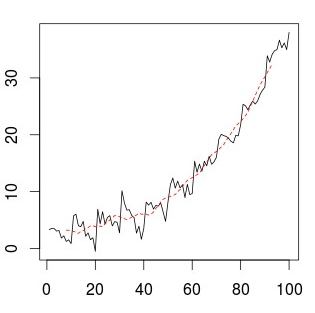
\includegraphics[width=90mm]{imagenes/moving_averages.png}
	\caption{Ejemplo algoritmo medias móviles.}
	\label{fig:51}
\end{figure}

Además de esto, también se pueden analizar los outliers que existan en la serie; si los outliers que se encuentren no aportan ninguna información adicional es mejor modificar su valor. También se podrían eliminar pero esto podría provocar una pérdida de información importante, por ello es mejor no hacerlo.\newline

Para la detección de outliers se puede utilizar cualquier método de detección de outliers univariable. Un método sencillo es el cálculo de outliers mediante IQR ( InterQuartile Range, rango intercuartílico en español ), para ello se calcula el IQR, el $Q_3$ y $Q_1$ el  de los datos para los cuales se quieren detectar outliers; se consideran outliers aquellos datos que estén fuera del rango definido por $[\ Q_1 - f*IQR, Q_3+f*IQR ]\ $ , donde $f$ es una constante.\newline

Normalmente $f$ suele tomar el valor $1.5$ , pero para el caso de las series temporales este valor provoca que se detecten demasiados datos como outliers; por ello, en este estudio se ha utilizado $f=3$ para asegurarse de que los outliers detectados sean realmente anomalías en los datos de la serie y no una pequeña variación. Una vez detectados los outliers, se pueden utilizar diferentes métodos para modificar dichos outliers, por ejemplo el método comentado anteriormente (medias móviles).\newline

Por último, se puede aplicar una selección de características, o en este caso de series temporales; para ello se pueden utilizar algoritmos de selección de características como por ejemplo Boruta \cite{kursa2010boruta}. Este algoritmo selecciona características dependiendo de su importancia. El proceso que sigue este algoritmo para seleccionar características se muestra en Algoritmo \ref{alg:boruta}.\newline

\begin{algorithm}[H]
	\caption{Boruta(C,N)}
	\label{alg:boruta}
	\begin{algorithmic}[0]
		\State \textbf{Entrada:} Conjunto de datos $C$, Número de iteraciones $N$.
		\State \textbf{Salida:} Conjunto de variables confirmadas $Confirmadas$.
		\State \textit{Confirmadas} = vector de atributos confirmados.
		\State \textit{Tentativas} = vector de atributos todavía sin confirmar ni rechazar.
		\State \textit{Rechazadas} = vector de atributos rechazados.
		\State \textit{Sombras} = vector para atributos duplicados.
		\State Tentativas = C.Atributos
		\For{$i \gets 1,N$}
			\State Añadir a Sombras todos los atributos en Tentativas.
			\State Mezclar de forma aleatoria cada uno de los Atributos de Sombras.
			\State Crear $C' = Tentativas \bigcup Sombras$
			\State Entrenar un clasificador RandomForest con el conjunto $C'$ y obtener la importancia de cada atributo.
			\ForAll{$attr \in Tentativas,sombra en Sombras$}
				\If{$importancia(attr) > importancia(sombra)$}
					\State $Confirmadas += attr$
				\Else
					\State $Rechazadas += attr$
				\EndIf
			\EndFor
		\EndFor
		\State return Confirmadas
	\end{algorithmic}
\end{algorithm}

\section{Método de la ventana}
Otro tipo de procesamiento que se propone es este trabajo es el uso de una ventana. El objetivo de utilizar este procesamiento es aprovechar la dependencia temporal que existe en las series temporales; es decir, los valores obtenidos en un instante (o para el caso de las series temporales de clasificación una clase) son dependientes de los $n$ valores anteriores.\newline
\newpage
Esta dependencia se utiliza en modelos clásicos de predicción de series temporales como es ARIMA. La Figura \ref{fig:52} muestra un ejemplo de predicción usando una ventana.\newline

\begin{figure}[H]
	\centering
	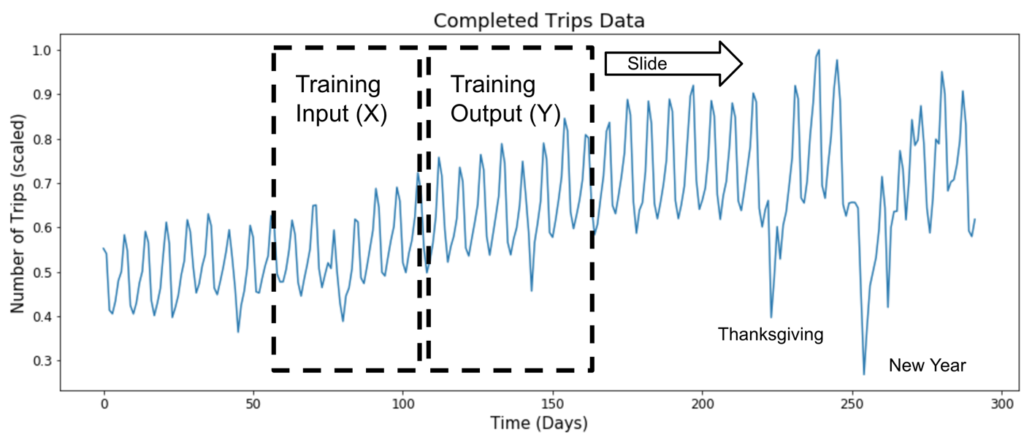
\includegraphics[width=100mm]{imagenes/sliding_window_ts.png}
	\caption{Ejemplo método de la ventana.}
	\label{fig:52}
\end{figure}
\verticalspace

Para los algoritmos clásicos de clasificación, así como las redes neuronales que se utilizan en este trabajo, no hay forma de que el modelo detecte dicha dependencia o se le pueda indicar directamente. Por ello, el procesamiento que se propone es replicar los datos anteriores, añadiéndolos como columnas a cada instancia, para replicar la misma ventana que se podría usar en un problema clásico de series temporales. El Algoritmo \ref{alg:wind_method} muestra el proceso para crear la ventana.\newline

\begin{algorithm}[H]
	\caption{Ventana(C,t)}
	\label{alg:wind_method}
	\begin{algorithmic}[0]
		\State \textbf{Entrada:} Conjunto de datos $C$, Tamaño de la ventana $t$.
		\State \textbf{Salida:} Conjunto de datos $C'$ con la ventana.
		\State $C'$ = conjunto de datos con la ventana creada.
		\ForAll{$attr \in C $}
			\For{$i \gets 0, t-1$}
				\State $C' = C' \bigcup desplazado(attr,i)$ // La función desplazado mueve hacia delante $i$ veces los datos de la columna $attr$.
			\EndFor
		\EndFor
		\State return $C'$
	\end{algorithmic}
\end{algorithm}
\verticalspace

Con este algoritmo se puede generar conjuntos de datos con una ventana añadida en cada columna, de forma que los algoritmos puedan hacer uso de la dependencia temporal. La Figura \ref{fig:53} muestra un ejemplo de dataset modificado por el algoritmo.\newline

\begin{figure}[H]
	\centering
	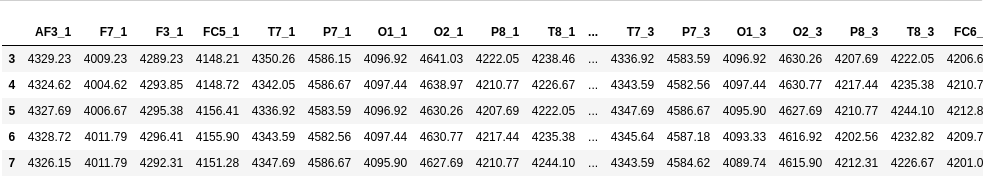
\includegraphics[width=130mm]{imagenes/ventana.png}
	\caption{Ejemplo de dataset modificado para tener una ventana de tamaño 3.}
	\label{fig:53}
\end{figure}
\verticalspace

Para obtener una mejora en el rendimiento, se debe estudiar que tamaño de ventana utilizar y este es diferente para cada conjunto de datos, aunque esto no se cubre dentro de este trabajo. Un aspecto a tener en cuenta cuando se utiliza es este algoritmo también es la dimensionalidad del conjunto de datos, ya que cuanto mayor es la ventana seleccionada mayor es el tamaño final del conjunto de datos y más costoso puede ser para un modelo procesarlo; además, un tamaño demasiado grande puede provocar sobreajuste, incluso empeorar el rendimiento.\newline




